% Testing Chapter

%% FIXME: Case study 1 (What, how, )

%%  * Describe test setup
%%  * For each case study - test case
%%  * Experiment -
%%    * clearly described test aim (What?)
%%    * How / What are the specifics of this test case / case study?
%%    * RESULTS
%%    * ANALYSIS


\section{Case Study 1}

% \subsection{What?}

The purpose of this case study is to identify network protocols used
in modern installation infrastructure system. In this case study a
service called netboot.xyz~\cite{netbootxyz} is used. Netboot.xyz is
free and open source service available from \url{https://netboot.xyz/}
and it's source code can be found from GitHub~\cite{github-netbootxyz}.

Netboot.xyz is used to install CentOS~7 Linux operating system. CentOS
Linux is community driven effort to provide free alternative to Red
Hat Enterprise Linux (RHEL). CentOS is built using RHEL source
code. Red Hat has 67 \% market share of Linux distribution market
according to Gartner's analysis~\cite{gartner-redhat}.

%% * Identify protocols used to achieve complete operating system installation.
%% * Use netboot.xyz installation infrastructure and CentOS 7.

% \subsection{How?}

The installation was done using virtual machine. VirtualBox was chosen
as a virtualization software because it's free, open source and has
easy to use network traffic recording functionality.

\begin{figure}[h]
  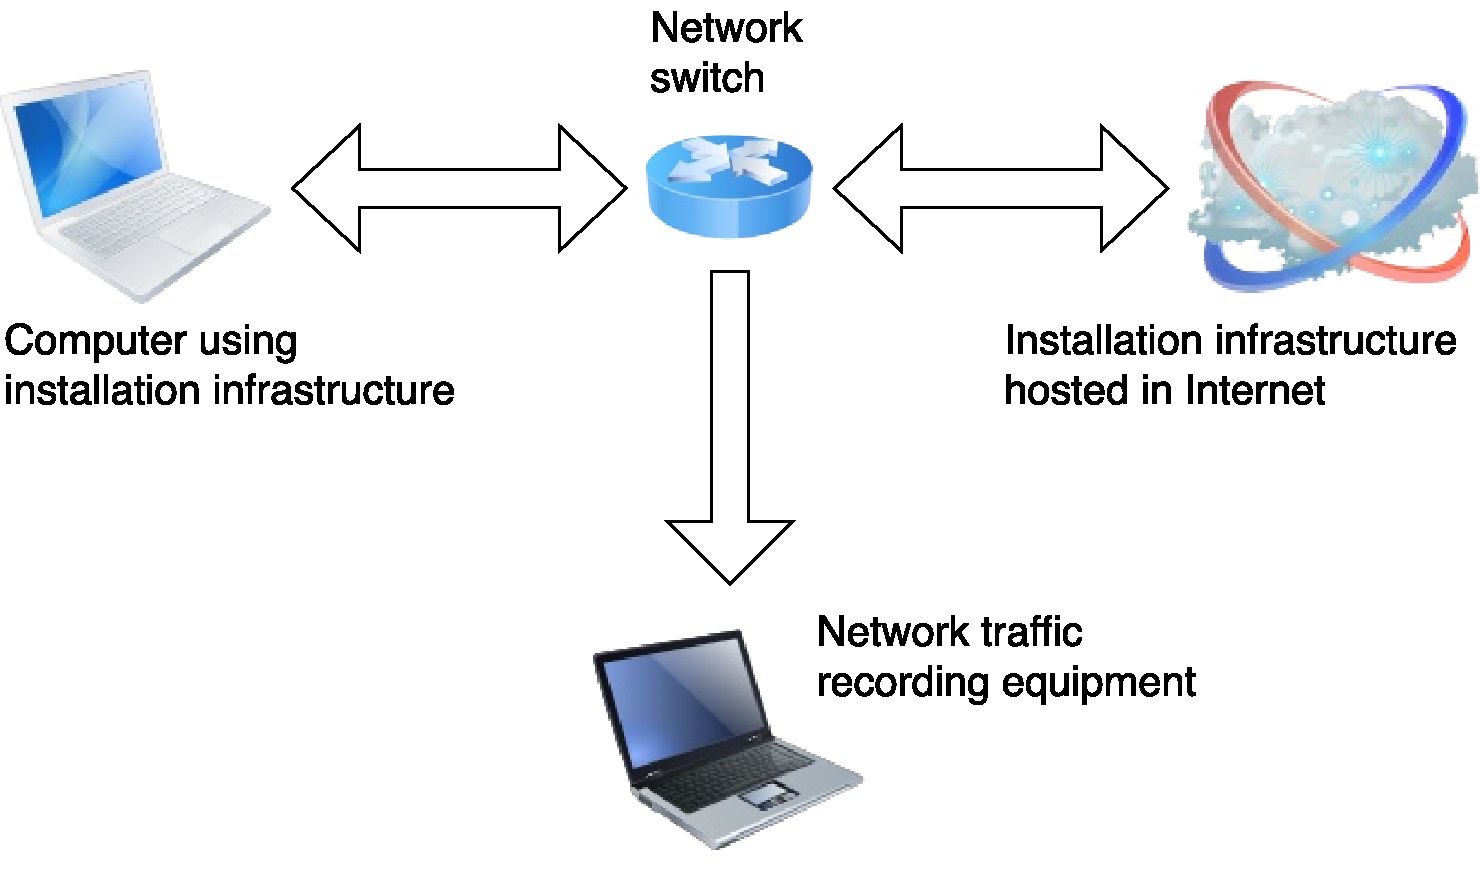
\includegraphics[width=\textwidth]{network-recording.pdf}
  \caption{Network traffic recording setup.\label{fig:network-recording}}
\end{figure}

With VirtualBox's netword traffic recording it's possible to get
network traffic captured for the whole lifetime of virtual
machine. The capture is saved as standard PCAP file which can later be
opened in network protocol
analyzer. Figure~\ref{fig:network-recording} has the typical traffic
capturing setup with computer using the installation infrastructure,
another computer recording the traffic, network switch to arrange
traffic flows and the Internet containing the installation
infrastructure in use.

Traffic capture is then analysed using Wireshark network protocol
analyzer. Wireshark is free and open source network protocol analyzer
which has capability to help user analyze many different network
protocols.

%% * VirtualBox installation
%% * VirtualBox's Network tracing
%% * Wireshark analysis

% \subsection{Results?}

Identified protocols in chronological order:

* DHCP
* ICMPv6 (Router Solicitation)
* ARP (Who has? router seeks client)
* Gratuitous ARP
* ARP (Who has? client seeks router)

\subsection{Analysis?}
